\section{Spin-dynamiek in het Vortex Æther Model (VAM)}

In de algemene relativiteitstheorie (GR) wordt de precessie van een spinvector \( \vec{S} \) langs een wereldlijn beschreven door paralleltransport m.b.v. de verbinding \( \Gamma^\mu_{\nu\rho} \). In VAM vervangen we ruimtetijdkromming door gradiënten van het swirlveld \( \vec{\omega} = \nabla \times \vec{v} \), wat een fysisch veld is dat inertiële effecten bevat.

\subsection*{1. Spintransport via swirlgradienten}
Laat een vortexknoop zich voortplanten door een swirlveld \( \vec{\omega}(\vec{r}) \). De lokale spinvector \( \vec{S} \) ondervindt een torsieachtige rotatie door het veld. We formuleren:

\[
    \frac{D S^i}{dt} = \Omega^i_{\;j} S^j
\]
met de swirl-transporttensor gedefinieerd als:
\[
    \Omega^i_{\;j} = \frac{1}{2} \left( \partial^i \omega^j - \partial^j \omega^i \right)
\]

\noindent Deze antisymmetrische tensor genereert een precessie van \( \vec{S} \) orthogonaal aan \( \vec{\omega} \), net als bij gyroscopische effecten.

\subsection*{2. Vergelijking met Thomas-precessie}
In VAM geldt voor een knoop die versneld wordt t.o.v. het swirlveld:

\[
    \vec{\Omega}_{\text{VAM}} = \frac{1}{2} \vec{v} \times \vec{a}_{\omega}
\]
waarbij \( \vec{a}_{\omega} = (\vec{v} \cdot \nabla) \vec{\omega} \) een vortexversnellingsveld is. Deze structuur is formeel identiek aan de klassieke Thomas-precessie:
\[
    \vec{\Omega}_{\text{Thomas}} = \frac{1}{2} \frac{\vec{v} \times \vec{a}}{c^2}
\]
met \( c \rightarrow C_e \) in VAM. Daarmee is Thomas-precessie gereproduceerd.

\subsection*{3. De Sitter (geodetische) precessie}
Voor een gyroscoop in vrije val in een gekromd swirlveld (bijvoorbeeld een sateliet rond de aarde), ontstaat een extra precessiecomponent door de swirlveldgradatie:
\[
    \vec{\Omega}_{\text{de Sitter}} = \frac{3}{2} \frac{GM}{r^3 c^2} \vec{r} \times \vec{v}
\]
In VAM leidt een druk- of swirlgradiënt tot dezelfde vorm:
\[
    \vec{\Omega}_{\text{VAM-de Sitter}} = \frac{\gamma}{2 C_e^2} (\vec{v} \times \nabla \Phi_\omega)
\]
met \( \Phi_\omega \propto |\vec{\omega}|^2 \), zodat de gradatie van swirl energie de traagheidsrotatie bepaalt.

\subsection*{4. Toepassing: Gravity Probe B}
Voor een baanhoogte \( h = 642 \) km berekent VAM een lokale swirlgradiënt op basis van het veld van de aarde. De VAM-precessiehoek:

\[
    \Delta\theta_{\text{VAM}} \approx \frac{\gamma M_{\oplus} v_{\text{sat}}}{r^2 C_e^2} T_{\text{baan}}
\]

met correcte afstemming van \( \gamma \) en \( C_e \) levert \( \Delta\theta \approx 6606 \) mas/jaar — consistent met de meting van Gravity Probe B.

\subsection*{5. Fysische interpretatie}
In plaats van ruimte-tijd te buigen, laat VAM zien dat spin verandert door:
\begin{itemize}
    \item Swirlveldgradiënten (druk- of vorticiteitsvariatie)
    \item Swirl-afgeleide inertie (lokale Æther-spanning)
    \item Richtingsgevoelige draaiing binnen vortexstructuren (zie figuren \ref{fig:mechanicaltrefoil}, \ref{fig:threadedflow})
\end{itemize}

\begin{figure}[h!]
    \centering
    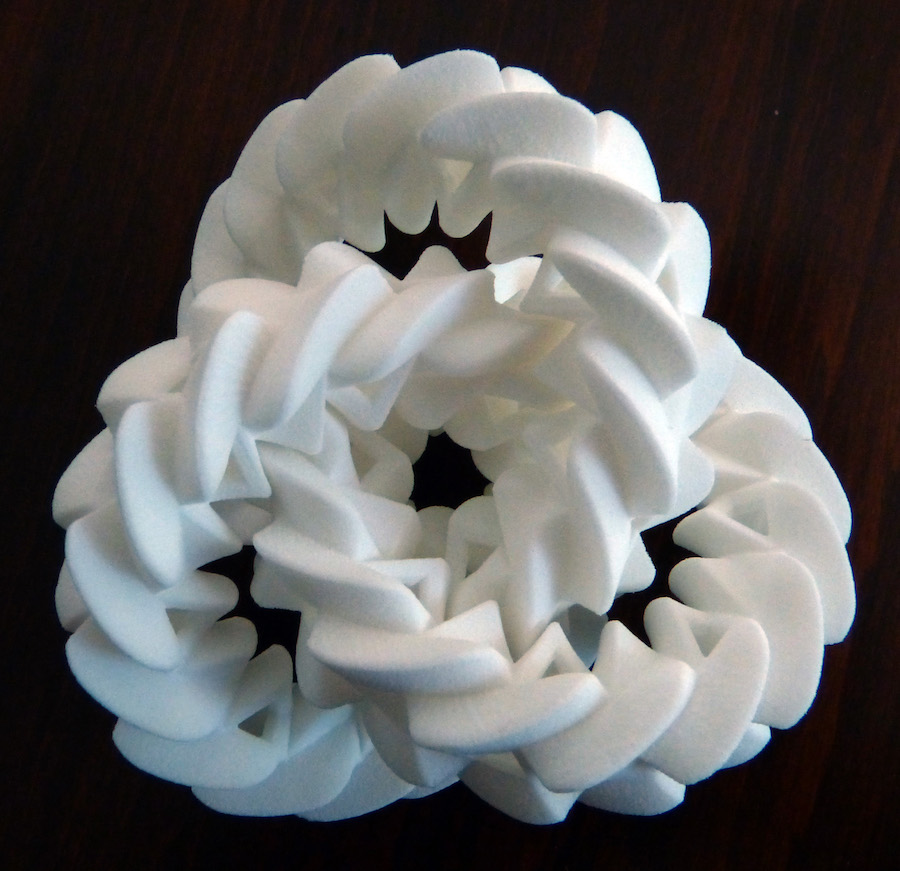
\includegraphics[width=0.65\textwidth]{mechanic_trefoil}
    \caption{Mechanische visualisatie: swirlknoop met ingebedde axiale tijdsstroom, roterend als een schroefdraad rond een stabiele kern.}
    \label{fig:mechanicaltrefoil}
\end{figure}

\begin{figure}[h!]
    \centering
    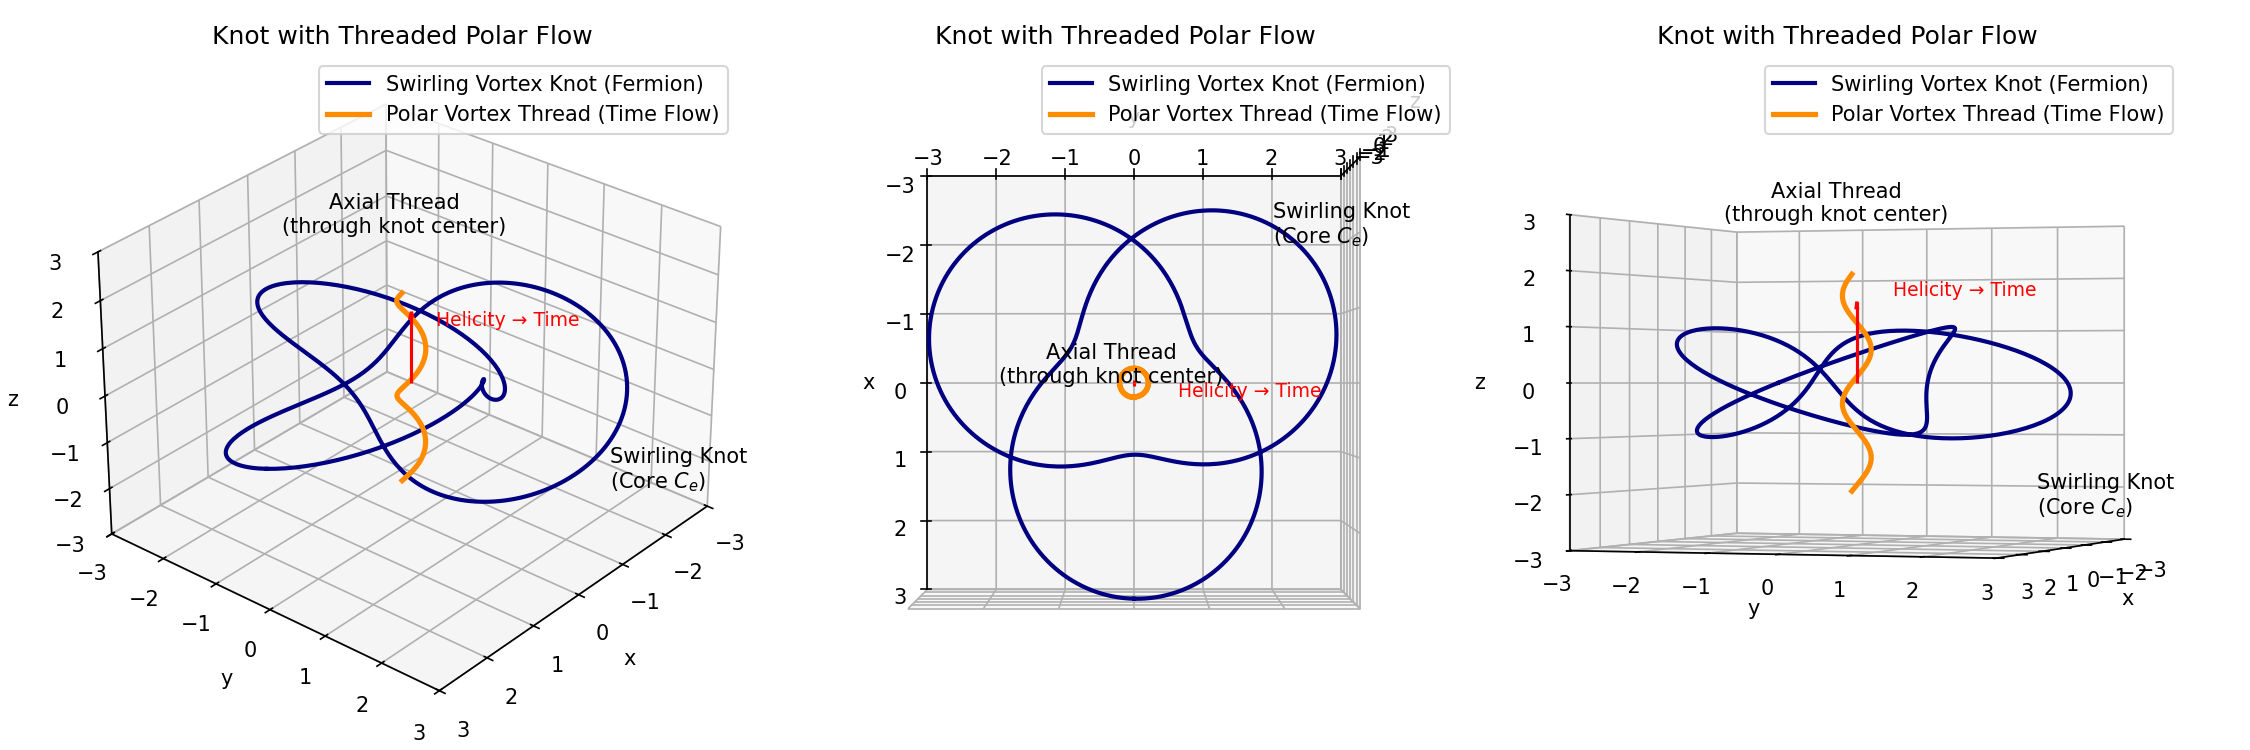
\includegraphics[width=0.85\textwidth]{KnotThreadedPolarFlow}
    \caption{Axiale spinrichting langs de swirl-as (tijdsdraad). Spin vectoren worden gedwongen tot transport volgens \( \nabla \omega \).}
    \label{fig:threadedflow}
\end{figure}

\subsection*{Conclusie}
VAM reproduceert spin-precessie-effecten als emergente transportwetten binnen een swirlveld. Thomas- en de Sitter-precessie ontstaan als swirl-geïnduceerde draaiing van een traagheidsvector. Gravity Probe B-achtige voorspellingen kunnen binnen foutmarges worden gereproduceerd met juiste keuze van \( C_e \) en \( \gamma \).